\documentclass{article}
\usepackage{polski}
\usepackage[utf8]{inputenc}
\usepackage[OT4]{fontenc}
\usepackage{graphicx,color}
\usepackage{url}
\usepackage[pdftex,hyperfootnotes=false,pdfborder={0 0 0}]{hyperref}
\usepackage{float}

\begin{document}
\thispagestyle{empty} %bez numeru strony

\begin{center}
{\large{Sprawozdanie z laboratorium:\\
Komunikacja człowiek–komputer}}

\vspace{3ex}

Przetwarzanie obrazu — aplikacja

\vspace{3ex}
{\footnotesize\today}

\end{center}


\vspace{10ex}

Prowadzący: dr hab.~inż. Maciej Komosiński

\vspace{5ex}

Autorzy:
\begin{tabular}{lllr}
\textbf{Sebastian Firlik} & inf122485 & sebastian.firlik@student.put.poznan.pl \\
\textbf{Adam Pioterek} & inf122446 & adam.pioterek@student.put.poznan.pl \\
\end{tabular}

\vspace{5ex}

Zajęcia czwartkowe, 15:10.

\vspace{35ex}

\noindent Oświadczam/y, że niniejsze sprawozdanie zostało przygotowane wyłącznie przez powyższych autora/ów,
a wszystkie elementy pochodzące z innych źródeł zostały odpowiednio zaznaczone i~są cytowane w bibliografii.  

\newpage



\section*{Udział autorów}
\begin{itemize}
\item Sebastian Firlik //TODO
\item Adam Pioterek — implementacja wykrywania samochodów na obrazie oraz ekstrahowania wielokątów zawierających samochody.
\end{itemize}

\section{Filtry i funkcje}
Do wykonania zadania wykorzystane zostały następujące filtry:
\begin{description}
\item[gaussian] — przeprowadza rozmycie Gaussa;\\
na wejściu otrzymuje zdjęcie w odcieniach szarości (macierz 2D) i odchylenie standardowe, na wyjściu daje macierz 2D – przefiltrowane zdjęcie.
Jego zadaniem jest rozmycie obrazu i tym samym pozbycie się niepotrzebnych i zaniedbywalnych szczegółów  a także szumów z naszego obrazu. Parametrem rozmycia Gaussa jest odchylenie standardowe $\sigma$ rozkładu normalnego. Im większe ono jest tym bardziej rozmyty jest obraz. W naszym programie $\sigma = 5$. 
\item[scharr] — odmiana filtru Sobela ze specjalnie dobranymi operatorami;\\
na wejściu funkcji musimy podać macierz z obrazem, gdzie w każdej komórce musi być jedna wartość (obraz w skali szarości, w jednym określonym kolorze). Opcjonalnie możemy podać maskę filtrowania. Wyjściem z funkcji jest przetransformowany obraz. Wybraliśmy filtr Scharra, ponieważ jest najbardziej niewrażliwy na rotację spośród innych dostępnych w bibliotece skimage (Sobel, Prewitt, Canny).
\item[dylatacja] — morfologiczna dylatacja, która powiększa jasne rejony na rzecz ciemnych;
na wejściu otrzymuje zdjęcie w odcieniach szarości (macierz 2D), na wyjściu daje macierz 2D.
\item[erozja] — morfologiczna erozja, która powiększa ciemne rejony na rzecz jasnych;
na wejściu otrzymuje zdjęcie w odcieniach szarości (macierz 2D), na wyjściu daje macierz 2D.
\end{description}
oraz funkcje:
\begin{description}
\item[threshold\_otsu] — progowanie Otsu, redukujące szarość do binarnego podziału na biel i czerń;\\
dzięki temu progowaniu otrzymaliśmy obraz biało-czarny, bez żadnych dodatkowych szarości. W ten sposób łatwiej nam było pozbyć się tła z obrazka.
\item[moments\_hu] — momenty Hu;\\
na wejściu otrzymuje znormalizowane momenty centralne, na wyjściu daje listę momentów Hu.
\item[ConvexHull] — otoczka wypukła;\\
na wejściu otrzymuje zbiór punktów, na wyjściu zwraca indeksy punktów należących do otoczki.
\end{description}

Wyjściem z ostatniej funkcji -- ConvexHull -- jest otoczka, którą przekształcamy w listę wierzchołków. Stanowią one wierzchołki wypukłego konturu samochodu. Następnie uruchamiamy naszą funkcję feature\_detection, której zadaniem jest uzyskać z danego na wejściu rozmiaru obrazka i konturu samochodu nasze cechy, opisane dalej.

Na końcu zapisujemy cechy, związane z każdym z obrazków do pliku CSV, co pozwala nam utworzyć w przyszłości zbiór uczący i testowy naszego klasyfikatora.

W pliku classify.py znajduje się skrypt, którego celem jest stworzenie drzewa decyzyjnego (CART), nauczenie go wzorców na podstawie naszych losowo wybranych danych treningowych, a następnie przetestowanie przykładów, które nie zostały użyte do procesu uczenia. Po zakończeniu działania programu otrzymujemy wizualizację drzewa decyzyjnego z podziałami na różnych atrybutach
 
\section{Cel eksperymentu}
Celem eksperymentu było stworzenie systemu rozpoznającego na zdjęciach samochody i kategoryzującego rozpoznane samochody jako sedan, suv lub van. //TODO
\section{Dane do eksperymentu}
//TODO pochodzenie danych
\begin{figure}[H]
\begin{center}
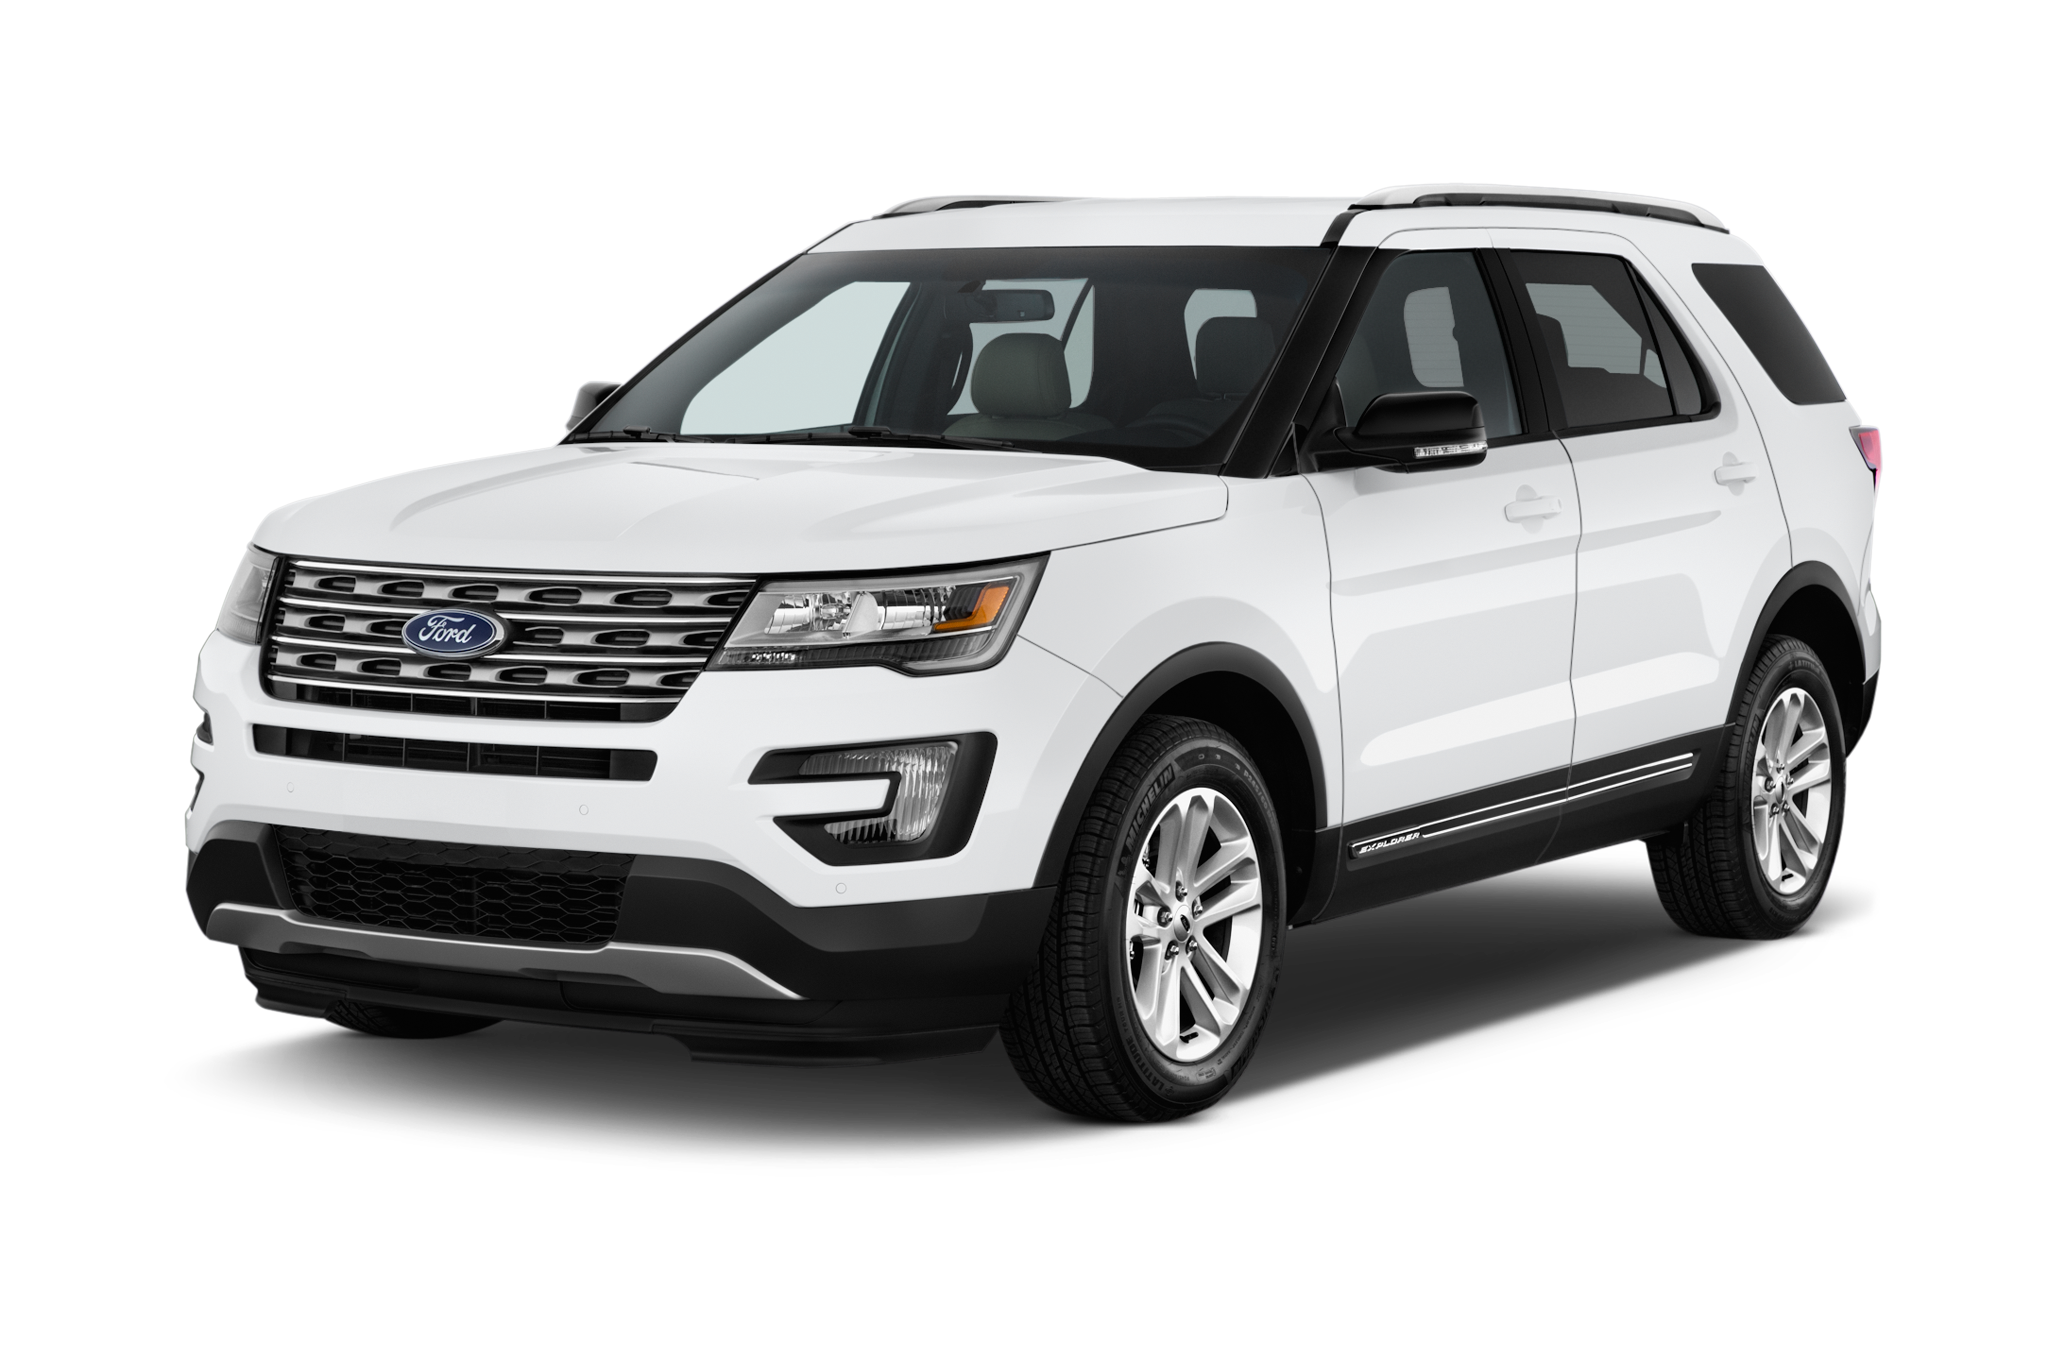
\includegraphics[width=1\textwidth]{../imgs_easy/suv_07.png}
\end{center}
\label{fig: wykres1}
\end{figure}
\begin{figure}[H]
\begin{center}
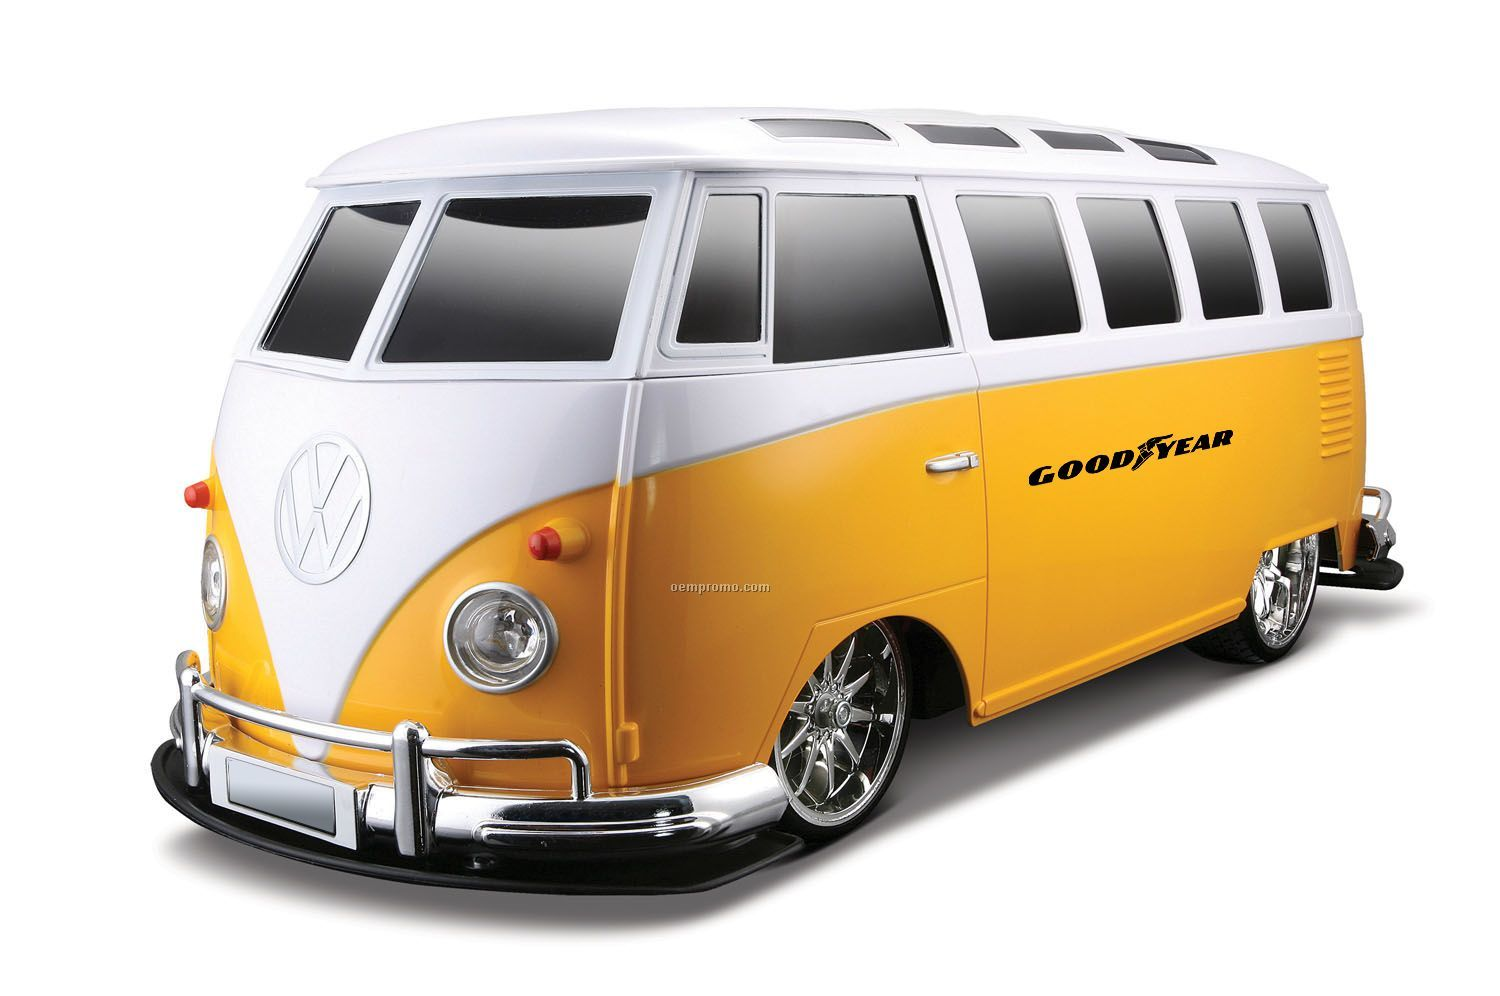
\includegraphics[width=1\textwidth]{../imgs_easy/van_19.jpg}
\end{center}
\label{fig: wykres2}
\end{figure}
\begin{figure}[H]
\begin{center}
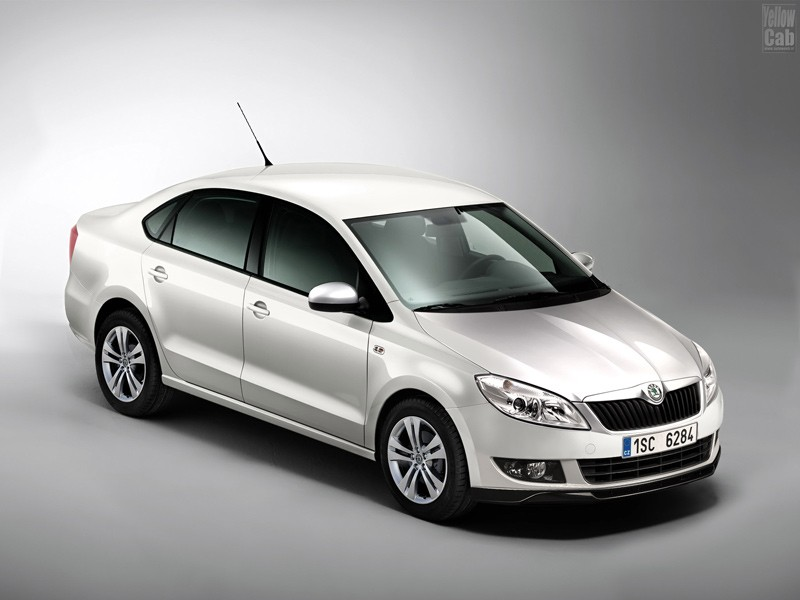
\includegraphics[width=1\textwidth]{../imgs_easy/sedan_22.jpg}
\end{center}
\label{fig: wykres3}
\end{figure}
\section{Efektywność}
Nasz program generował 12 atrybutów warunkowych i 1 atrybut decyzyjny dla każdego obrazka. Atrybut decyzyjny miał jedną z trzech wartości ze zbioru ${d, s, v}$, odpowiednio dla samochodów typu sedan, suv i van. Natomiast pośród atrybutów warunkowych możemy wyróżnić:
\begin{enumerate}
\item Siedem momentów Hu
\item Stosunek obwodu otoczki wypukłej samochodu do jej pola
\item Znormalizowana wysokość konturu -- osiągnęliśmy to dzięki podzieleniu różnicy maksimum i minimum współrzędnych \textit{y} przez wysokość całego obrazka w pikselach.
\item Stosunek wysokości samochodu do jego długości
\item Stosunek pola powierzchni samochodu do pola całego obrazka
\item Liczba wierzchołków otoczki wypukłej samochodu -- wklęsłe wierzchołki przy oponach samochodów zostały usunięte w procesie tworzenia otoczki, jednak nie wpływa to negatywnie na ważność tej cechy, ponieważ każdy samochód ma te wierzchołki, więc możemy je od każdego przykładu odjąć.
\end{enumerate}

\end{document}
